\documentclass[final]{beamer}


% <<< packages
\usetheme[size=a1, orientation=landscape, scale=1.0, nomyriadpro]{uvtposter}

\headerdepartment{Master Bioinformatică}
\headerconference{Susținere disertație --- Iulie 2026}

\usepackage{amsmath}
\usepackage{hyperref}
\usepackage{booktabs}
\usepackage{graphicx}
\usepackage{multirow}
\usepackage{tabularx}
\usepackage{tikz}
\usetikzlibrary{shapes.geometric, arrows.meta, positioning}

\newcommand{\tikzmark}[1]{\tikz[remember picture, baseline] \node[inner sep=0pt, outer sep=0pt] (#1) {};}

% >>>

% <<< metadata

\title{Identificarea automată a speciilor de raci din genul\\[0.5em]
       \textit{Austropotamobius}\\[0.5em]
       prin tehnici de deep learning pe bază de imagini}

\author{\underline{Smarandache Grigorie Theodor} \\[0.3em]
        \small Coordonatori: Prof. dr. Habil. Zaharie Daniela, Prof. dr. Habil. Pârvulescu Lucian}

\institute[shortinst]{Facultatea de Informatică, Universitatea de Vest din Timișoara}

\footerweb{https://info.uvt.ro/}
\footerlocation{Facultatea de Informatică, Universitatea de Vest din Timișoara --- Iulie 2026}
\footeremail{grigorie.smarandache02@e-uvt.ro}

% >>>

\begin{document}

\begin{frame}[fragile]

\begin{columns}[t]
\begin{column}{0.015\paperwidth}\end{column}

% ===================== COLOANA 1 =====================
\begin{column}{0.3\paperwidth}

\begin{block}{Motivație și context}

Racii de apă dulce din genul \textit{Austropotamobius} sunt specii
\textbf{protejate}, reprezentând indicatori valoroși ai calității
habitatelor acvatice. Identificarea corectă a speciilor
\textit{A.~bihariensis} și \textit{A.~torrentium} este dificilă din
cauza similarității morfologice pronunțate.

\smallskip

\textbf{Scop:} identificarea automată a speciei de rac și discriminarea
între \textit{A.~b.} și \textit{A.~t.} pe baza imaginilor de teren.

\smallskip

\textbf{Provocări:}
\begin{itemize}
    \item Similarități pronunțate: crustă netedă, creastă postorbitală
          discretă, rostru triunghiular
    \item Diferențe vizibile doar în detalii fine (lungimea solzului
          antenal, rugozitatea chelelor)
    \item Variabilitate între specii mare de colorit la \textit{A.~t.}
    \item Identificarea manuală depinde de experiența evaluatorului
\end{itemize}

\smallskip

\begin{figure}
    \centering
    \begin{minipage}{0.42\linewidth}
        \centering
        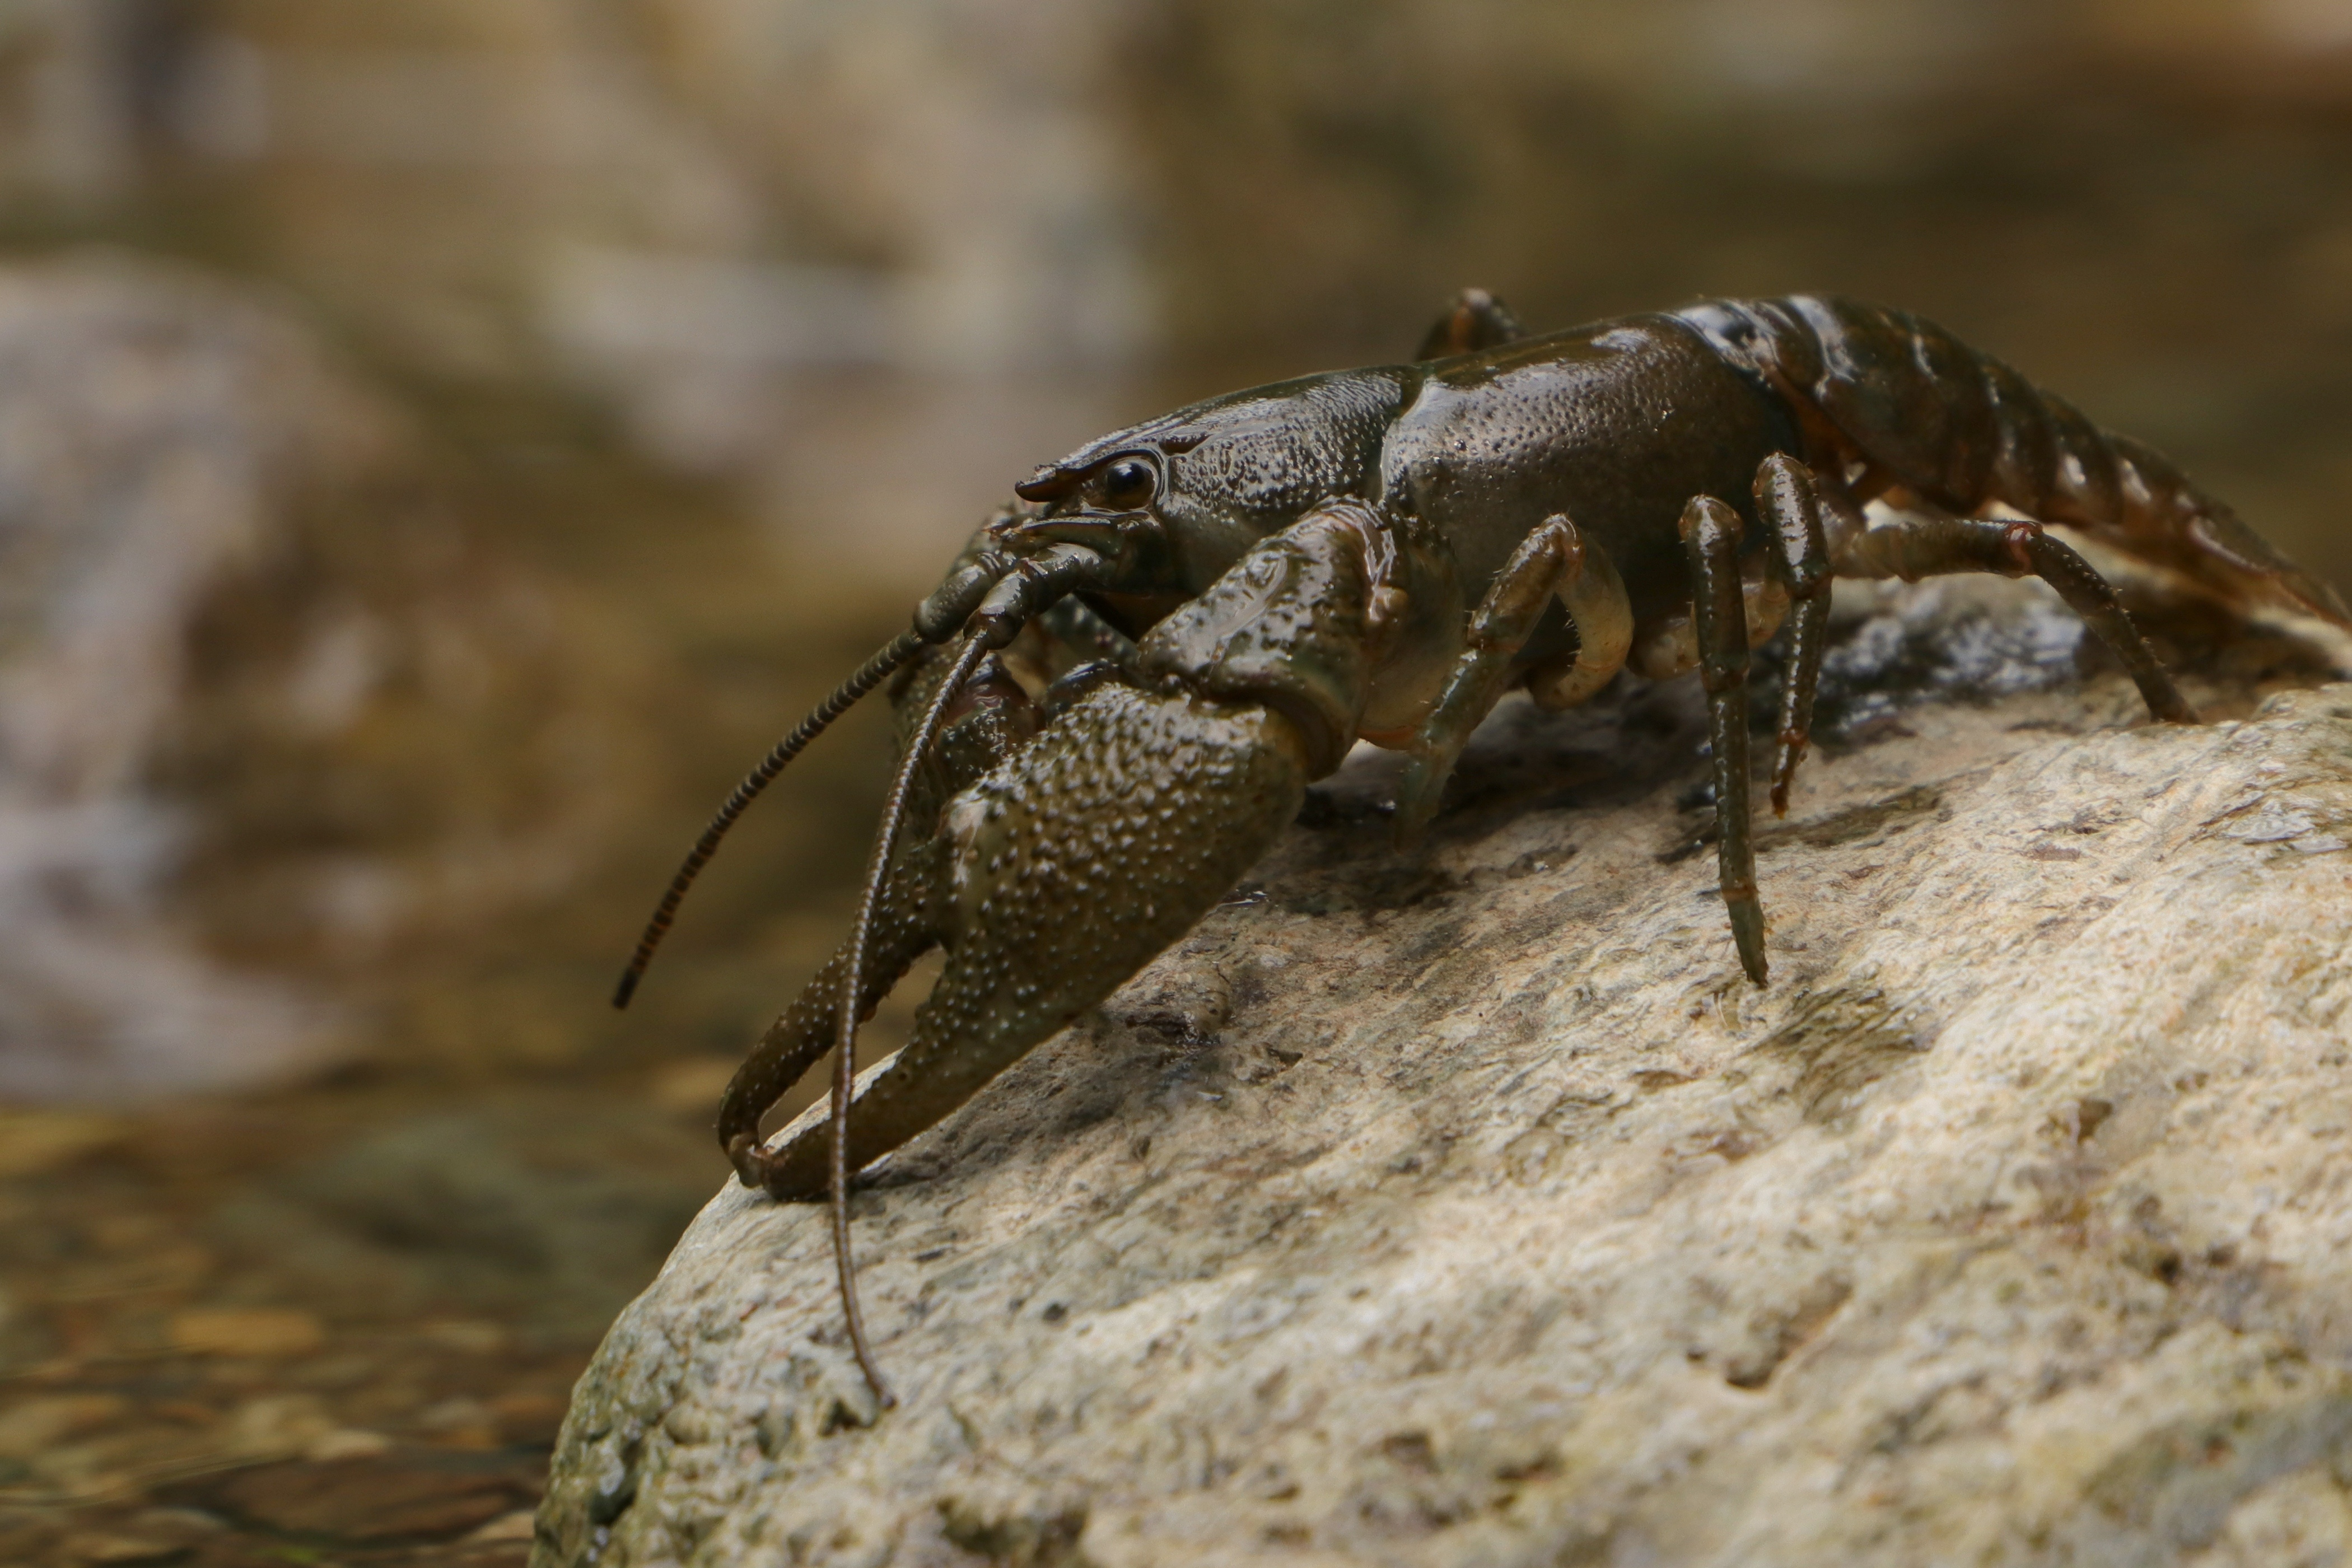
\includegraphics[width=\linewidth]{assets/Bihariensis_ex1_resize.jpg}\\[3pt]
        {\large \textit{A.~bihariensis}}
    \end{minipage}
    \hspace{0.5em}
    \begin{minipage}{0.42\linewidth}
        \centering
        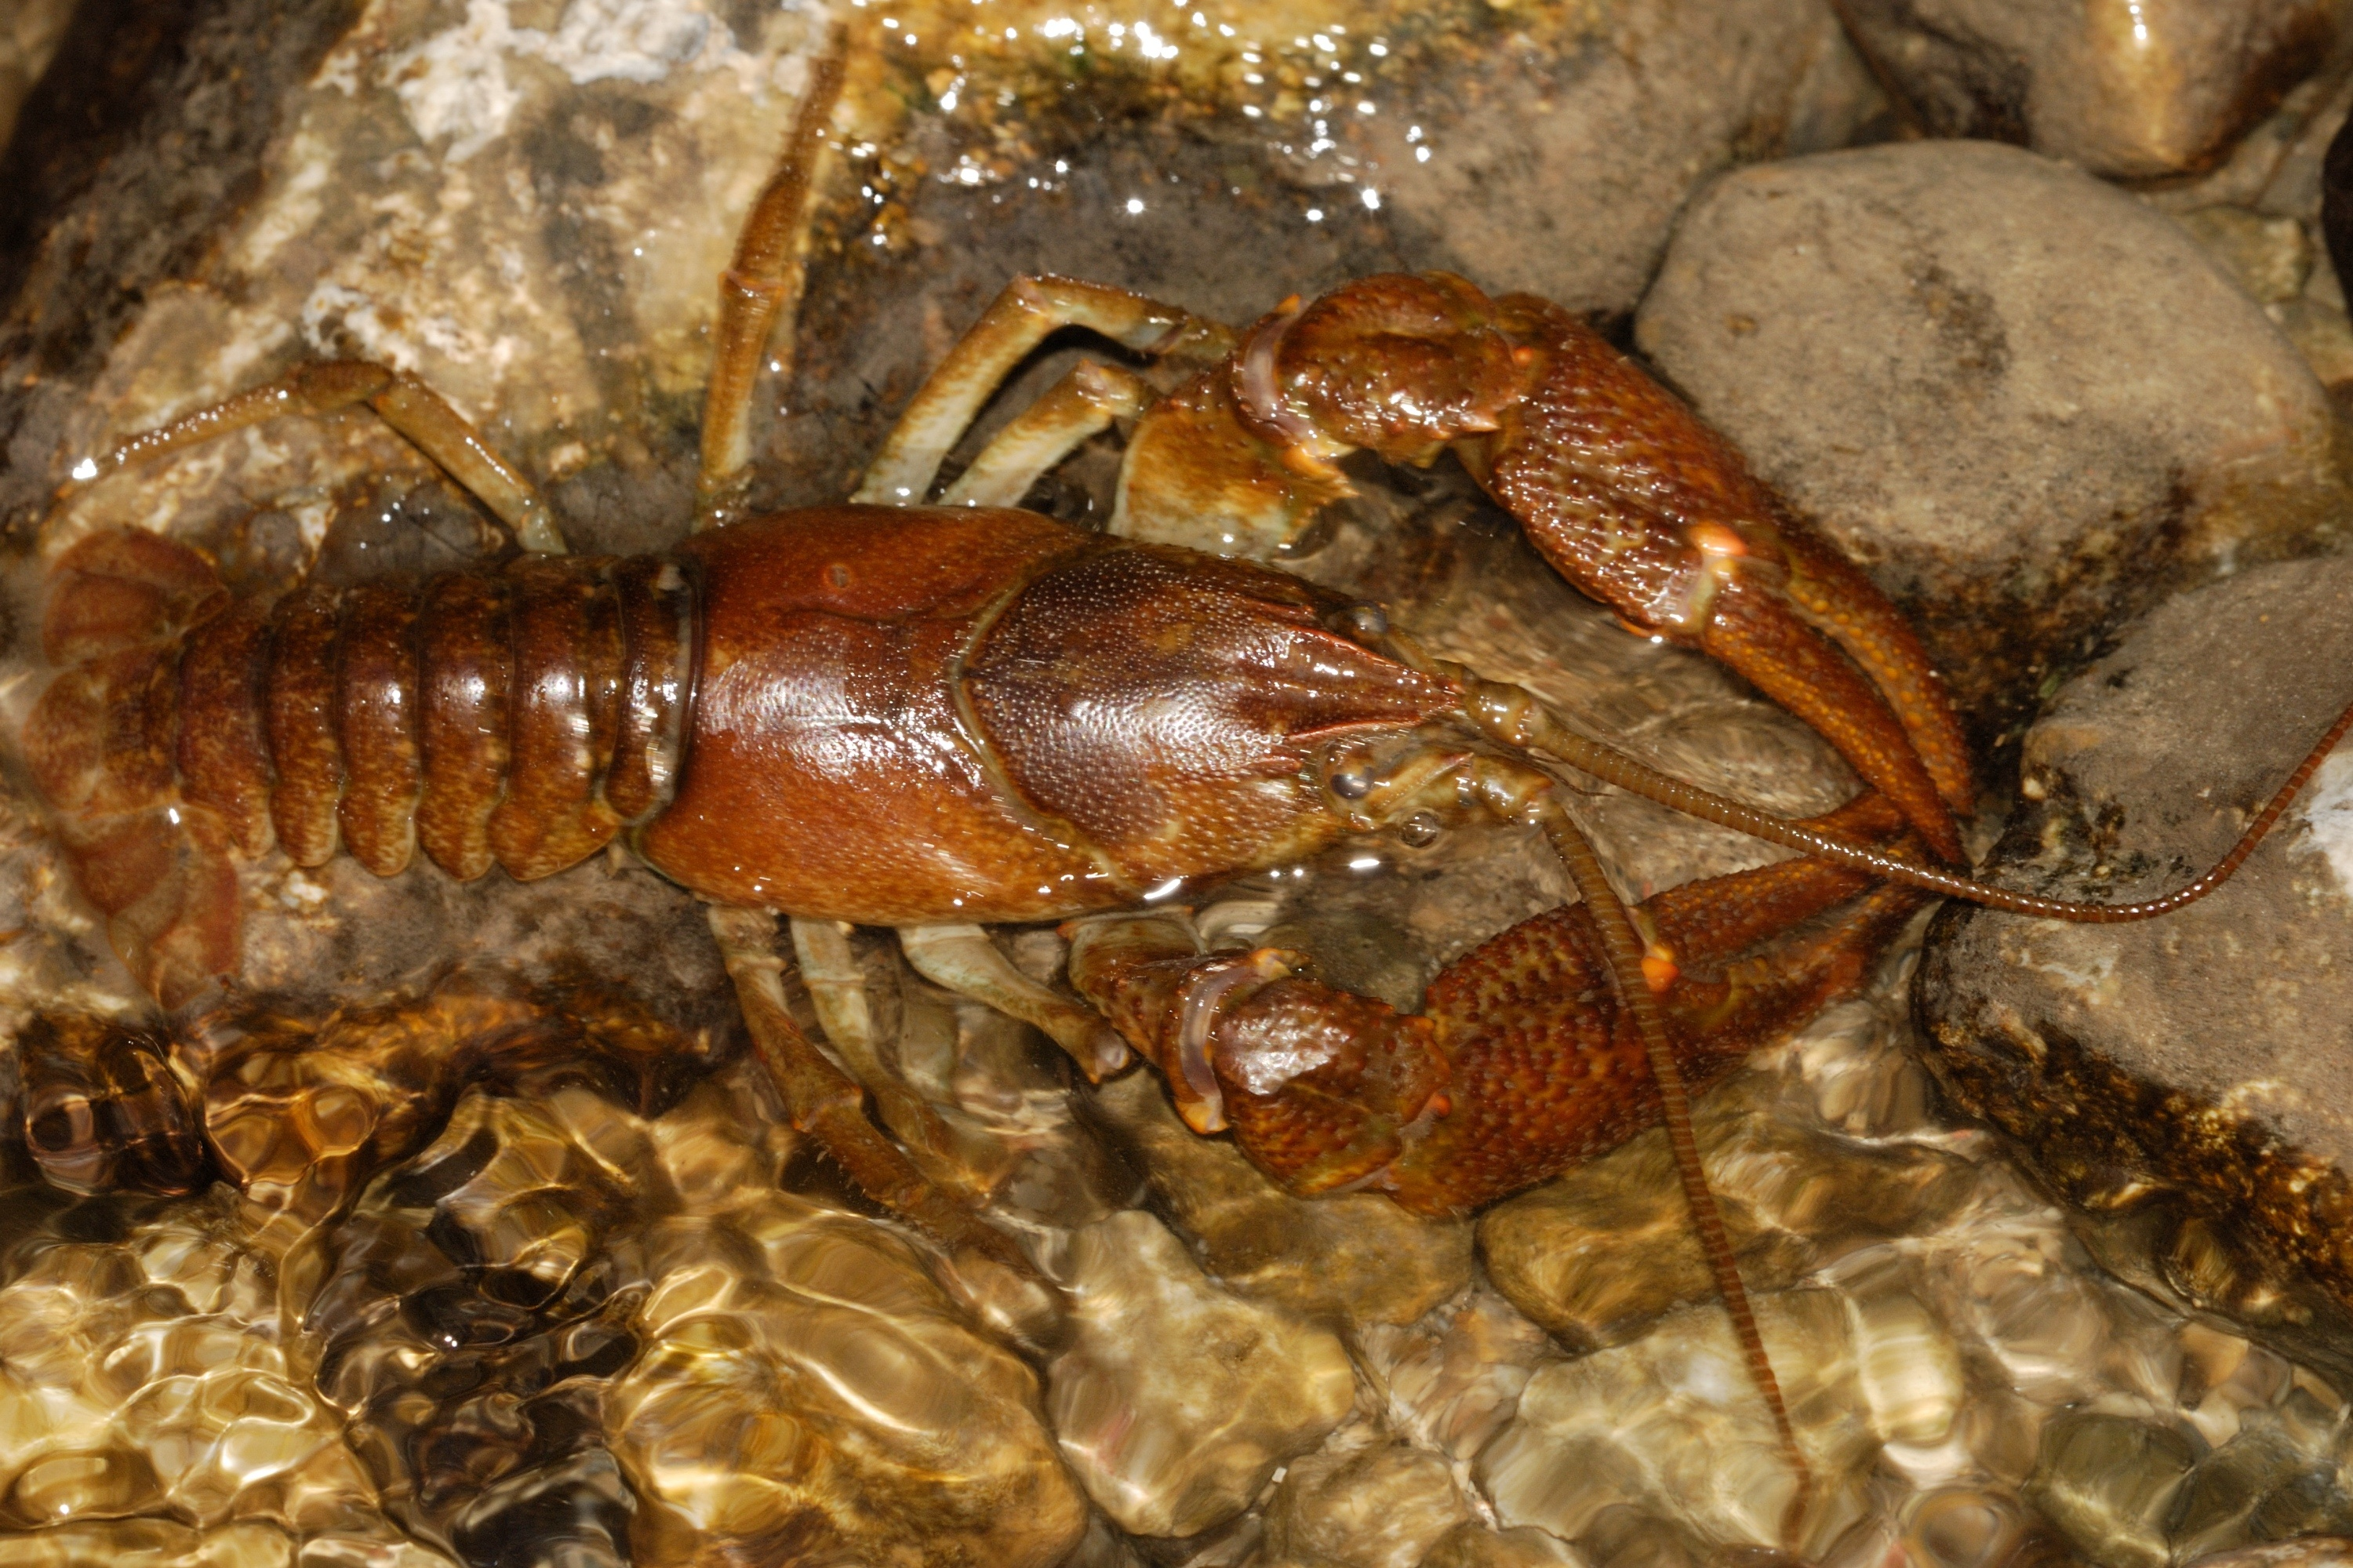
\includegraphics[width=\linewidth]{assets/Torrentium_ex1_resize.jpg}\\[3pt]
        {\large \textit{A.~torrentium}}
    \end{minipage}
\end{figure}

\end{block}

\begin{block}{Setul de date}

\begin{table}
\centering
\begin{tabular}{@{} lcc @{}}
    \toprule
    \textbf{Specie} & \textbf{Imagini} & \textbf{Procent} \\
    \midrule
    \textit{A.~bihariensis} & 182 & 57,2\% \\
    \textit{A.~torrentium}  & 136 & 42,8\% \\
    \midrule
    \textbf{Total}          & \textbf{318} & \textbf{100\%} \\
    \bottomrule
\end{tabular}
\end{table}

\smallskip

Set propriu, colectat din teren, adnotat manual cu LabelMe
\cite{labelme} (bounding box, eticheta \texttt{rac}).
Împărțire stratificată: 70\% / 15\% / 15\% (\texttt{seed=42}).

\end{block}

\begin{block}{Flux de prelucrare}

\smallskip

\begin{center}
\begin{tikzpicture}[
    node distance=1.3cm and 1.5cm,
    box/.style={rectangle, rounded corners=8pt,
                minimum width=8.2cm, minimum height=3.4cm,
                align=center, font=\Large\bfseries, inner sep=12pt},
    arrow/.style={-{Stealth[length=10pt, width=9pt]}, line width=3pt, color=UVTDarkBlue}
]
    \node[box, draw=UVTDarkBlue, fill=UVTDarkBlue, text=white] (ann)
        {1. Adnotare manuală\\[6pt]
         {\normalsize\mdseries LabelMe --- bounding box}};

    \node[box, draw=UVTDarkBlue!70, fill=UVTLightBlue!50, text=UVTDarkBlue,
          below=of ann] (roi)
        {2. Extragere ROI\\[6pt]
         {\normalsize\mdseries decupare automată --- 227$\times$227~px}};

    \node[box, draw=UVTPosterYellow!90!black, fill=UVTPosterYellow!50, text=UVTDarkBlue,
          below=of roi] (aug)
        {3. Augmentare date\\[6pt]
         {\normalsize\mdseries flip, rotație, culoare, blur}};

    \node[box, draw=UVTDarkBlue, fill=UVTLightBlue!80, text=UVTDarkBlue,
          right=of aug] (train)
        {4. Construire model\\[6pt]
         {\normalsize\mdseries AlexNet + transfer learning}};

    \node[box, draw=UVTDarkBlue!50!green!80, fill=UVTDarkBlue!15, text=UVTDarkBlue,
          above=of train] (eval)
        {5. Evaluare\\[6pt]
         {\normalsize\mdseries acuratețe, precizie, recall, F1}};

    \draw[arrow] (ann)   -- (roi);
    \draw[arrow] (roi)   -- (aug);
    \draw[arrow] (aug)   -- (train);
    \draw[arrow] (train) -- (eval);

\end{tikzpicture}
\end{center}

\end{block}

\end{column}

\separatorcolumn

% ===================== COLOANA 2 =====================
\begin{column}{0.3\paperwidth}

\begin{block}{Augmentarea datelor}

Augmentări aplicate la antrenare: flip orizontal/vertical, rotație,
schimbare de perspectivă, decupare (crop) medie, variație de culoare,
blur Gaussian, ștergere aleatorie de regiuni.

\smallskip

\begin{figure}
    \centering
    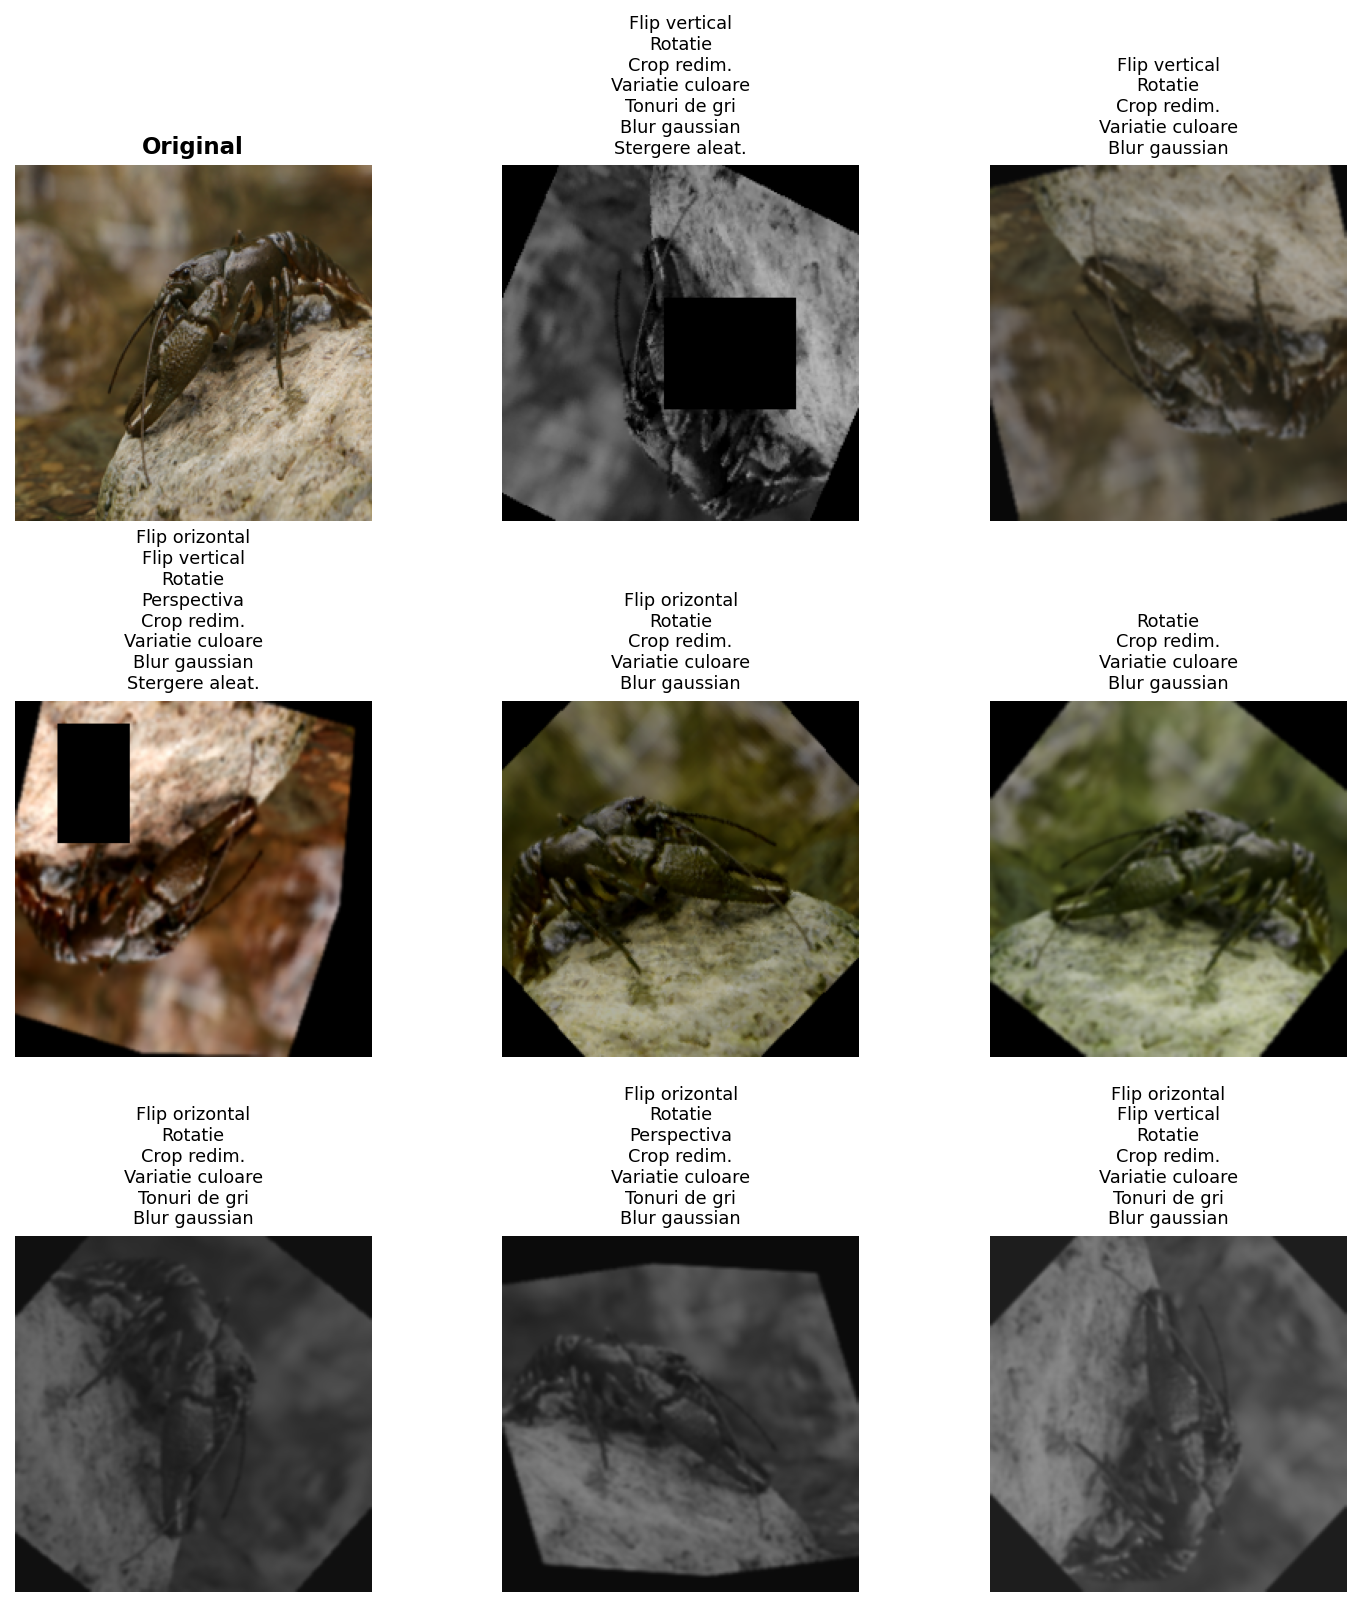
\includegraphics[width=0.62\linewidth]{assets/AugmentariGridBihariensis.png}
\end{figure}

\end{block}

\begin{block}{AlexNet + transfer learning}

Modelul utilizat este \textbf{AlexNet} \cite{krizhevsky2012imagenet},
pre-antrenat pe ImageNet (1,2M imagini, 1000 clase), adaptat pentru
clasificare binară prin:

\begin{itemize}
    \item \textbf{Straturile convoluționale} sunt înghețate ---
          se păstrează reprezentările vizuale din ImageNet
    \item \textbf{Straturile complet conectate} (FC6--FC8) sunt
          reantrenate pentru cele 2 clase
\end{itemize}

\smallskip

\noindent\hspace*{\fill}
\begin{minipage}{0.44\linewidth}
    \centering
    \normalsize
    \begin{tabular}{@{} llc @{}}
        \toprule
        \textbf{Strat} & \textbf{Tip} & \textbf{Antrenat} \\
        \midrule
        1 & Convoluție & Nu \\
        2 & Convoluție & Nu \\
        3 & Convoluție & Nu \\
        4 & Convoluție & Nu \\
        5 & Convoluție & Nu \\
        6 & FC (4096)  & \textbf{Da} \\
        7 & FC (4096)  & \textbf{Da} \\
        8 & FC (2)     & \textbf{Da} \\
        \bottomrule
    \end{tabular}
\end{minipage}
\hspace{0.02\linewidth}
\begin{minipage}{0.44\linewidth}
    \centering
    \normalsize
    \begin{tabular}{@{} ll @{}}
        \toprule
        \textbf{Hiperparametru} & \textbf{Valoare} \\
        \midrule
        Optimizator       & SGD \\
        Rată de învățare  & 0,001 \\
        Momentum          & 0,9 \\
        Weight decay      & 0,0005 \\
        Label smoothing   & 0,1 \\
        Dimensiune batch  & 32 \\
        Număr epoci       & 60 \\
        Scheduler         & ReduceLROnPlateau \\
        \bottomrule
    \end{tabular}
\end{minipage}
\hspace*{\fill}

\end{block}

\begin{block}{Rezultate}

Modelul final obține \textbf{95,92\% acuratețe} pe setul de testare
independent (47 din 49 imagini clasificate corect).

\smallskip

\begin{table}
\centering
\normalsize
\begin{tabular}{@{} lccc @{}}
    \toprule
    \textbf{Clasă} & \textbf{Precizie} & \textbf{Recall} & \textbf{F1} \\
    \midrule
    \textit{A.~b.} & 0,9643 & 0,9643 & 0,9643 \\
    \textit{A.~t.} & 0,9524 & 0,9524 & 0,9524 \\
    \midrule
    \textbf{Macro} & 0,9583 & 0,9583 & \textbf{0,9583} \\
    \bottomrule
\end{tabular}
\end{table}

\end{block}

\end{column}

\separatorcolumn

% ===================== COLOANA 3 =====================
\begin{column}{0.3\paperwidth}

\begin{block}{Evoluția performanței}

Acuratețea a crescut progresiv pe parcursul celor \textbf{4 configurații}.

\smallskip

\begin{table}
\centering
\begin{tabularx}{0.98\linewidth}{@{} c c X c @{}}
    \toprule
    \textbf{Config.} & \textbf{Acuratețe} & \textbf{Îmbunătățire principală} & \textbf{Batch} \\
    \midrule
    1 & 62,50\% & Baseline --- împărțire 70\%/15\%/15\% & 32 \\
    2 & 87,50\% & Augmentare date, îngheațarea straturilor convoluționale, normalizare ImageNet (medie/std) & 32 \\
    3 & \textcolor{UVTDarkBlue}{\textbf{95,92\%}} & Extragere automată ROI (crop) & 32 \\
    4 & 93,88\% & Batch 64 (performanță mai scăzută) & 64 \\
    \bottomrule
\end{tabularx}
\end{table}

\end{block}

\begin{block}{Predicții}

\begin{figure}
    \centering
    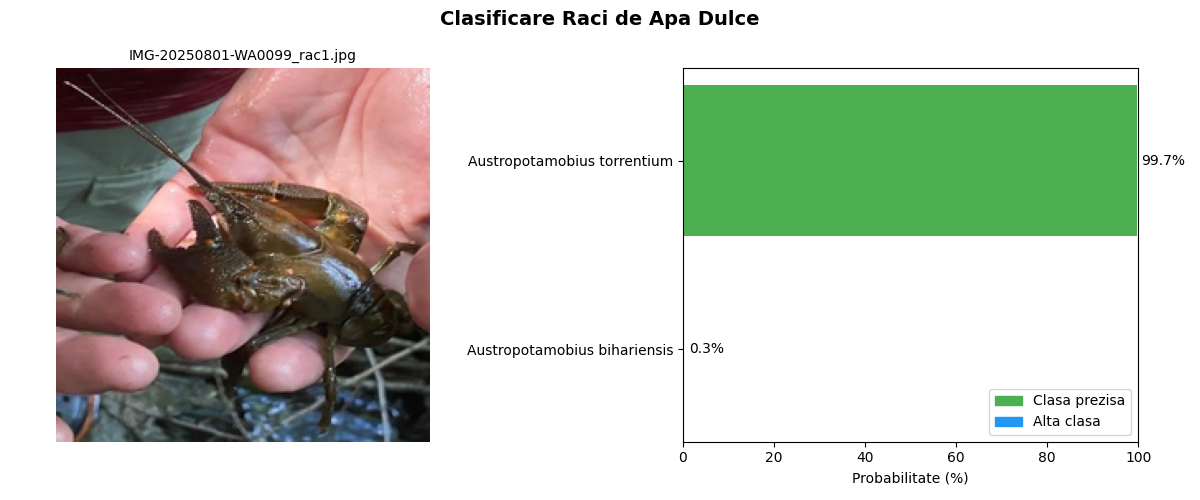
\includegraphics[width=0.54\linewidth]{assets/Pred1_FoarteMare_Torrentium.png}\\[4pt]
    {\footnotesize  \textit{A.~t.} --- 99,7\% confidence}

    \bigskip

    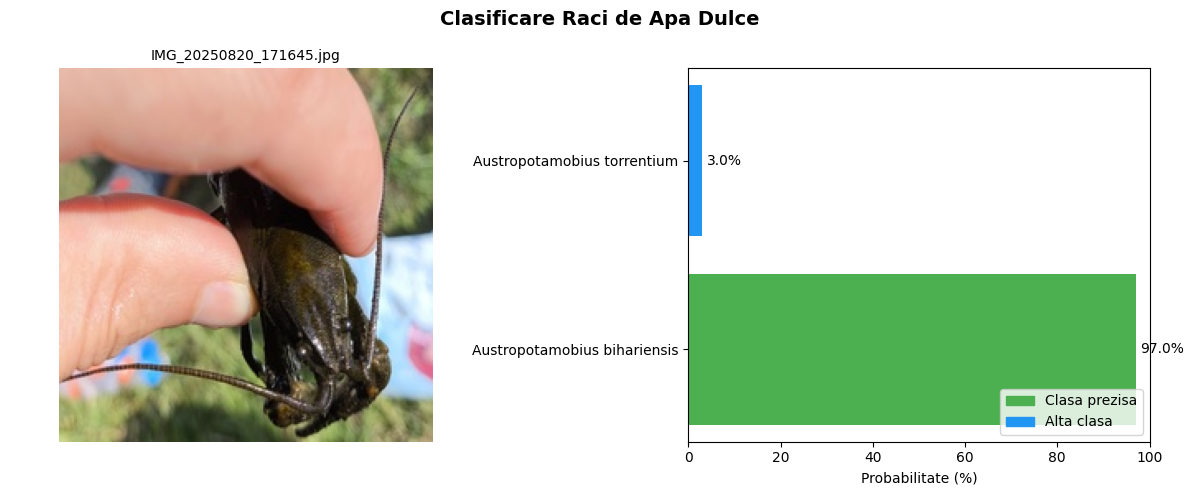
\includegraphics[width=0.54\linewidth]{assets/Pred2_Mare_Bihariensis.png}\\[4pt]
    {\footnotesize  \textit{A.~b.} --- 97,0\% confidence}
\end{figure}

\end{block}

\begin{exampleblock}{Comparație cu abordări existente}

Lucrări recente abordează identificarea automată a racilor
(\textit{Procambarus clarkii}) cu arhitecturi YOLO
\cite{shi2024lightweight,islam2024identification,geng2024application}.
Față de acestea:

\begin{itemize}
    \item Clasificare între specii, nu detecție anatomică
    \item Două specii \emph{protejate}, morfologie similară
    \item Imagini de teren, fundal și iluminare variabile
    \item Doar 318 imagini --- mult mai puține
\end{itemize}

\smallskip

Transfer learning-ul din ImageNet folosind AlexNet este viabil pentru seturi de date mici.

\end{exampleblock}

\begin{alertblock}{Referințe}

\hfill\tikzmark{qrcorner}\par\vspace{-\baselineskip}
\footnotesize
\bibliographystyle{unsrt}
\bibliography{poster}

\end{alertblock}

\begin{tikzpicture}[remember picture, overlay]
    \node[anchor=north east, xshift=-0.2cm, yshift=0.2cm] at (qrcorner) {
\includegraphics[width=2.6cm]{assets/qrcode.png}};
\end{tikzpicture}

\end{column}

\begin{column}{0.015\paperwidth}\end{column}
\end{columns}
\end{frame}

\end{document}